\documentclass[twocolumn]{article}
\usepackage{multicol}
\usepackage{geometry}% http://ctan.org/pkg/geometry
\usepackage{lipsum}% http://ctan.org/pkg/lipsum
\usepackage{graphicx}% http://ctan.org/pkg/graphicx
\usepackage{blindtext}
\usepackage{ltablex}% <-- added
\usepackage{siunitx}% <-- added
\usepackage{caption}% <-- added 
\usepackage{booktabs,siunitx}
\usepackage{varwidth}
\usepackage{makecell}
\usepackage{stfloats}
\usepackage{hanging}
\usepackage[
  justification=RaggedRight,
  calcwidth=.9\linewidth,
]{caption}
\newcommand\tab[1][1cm]{\hspace*{#1}}
%set margins
\geometry{
    left=2cm,
    right=2cm,
    top=1.5cm,
    bottom=1.5cm,
}
\setlength{\columnsep}{0.8cm}
\begin{document}


\twocolumn[
    \begin{@twocolumnfalse}
        \begin{center}
            \Large\textbf{A Designed Insect Trap Annotation Pipeline on Macleish}\\
      \large\textit{Sanjana Yasna (Teetly)}
         \end{center}
     \end{@twocolumnfalse}

\bigskip]
\section{Introduction}
    \tab Moths serve as indicator species for biodiversity. To assess ecological health, 
    Mariana Abarca and her lab collect insect samples using light-based traps at Macleish. 
    However, these traps can disorient insects and interfere with their natural behaviors. 
    To minimize this disruption, the lab wants to know the peak time of insect activity 
    so that traps can be deployed briefly—a few dozen minutes a day, if possible. \newline
    \tab In an ideal scenario, traps would be set when moth activity is highest. However, due to the 
    lack of annotations on the Macleish image dataset, it's not possible to confidently determine 
    when most moths land. Instead, this project uses the total number of detected insects 
    as a proxy.  Detected insects were still classified as moths or non-moths using a model fine-tuned on 
    external, 
    labeled crops of insects from trap images.  Classifier predictions were logged to enable manual evaluation 
    of predictions by Mariana and her lab so they can give insights on model weaknesses.
    Additionally, due to the model's excellent performance on the proxy traps dataset,
    there is proof-of-concept that a model can reliably detect moths 
    on the Macleish images if given sufficient labels to train on.
    \newline
    \begin{figure}[!t]
        \begin{varwidth}{0.5\textwidth}
            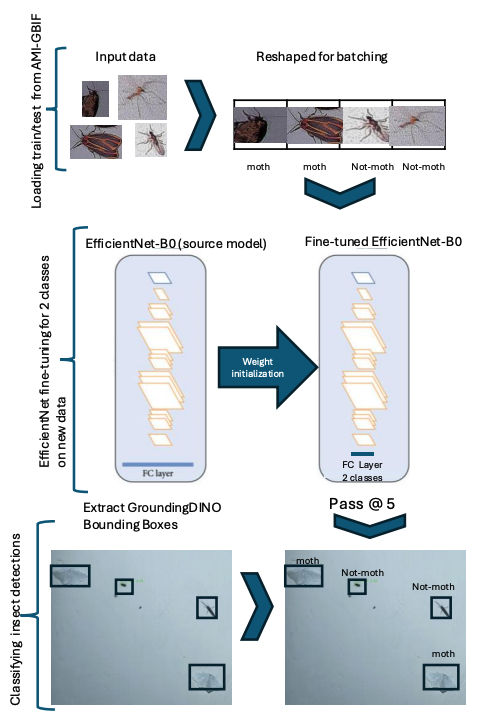
\includegraphics[width=9cm, height=13cm]{imgs/try.png}
            \captionsetup{width=0.9\textwidth}
            \caption*{\textbf{Figure 1:} Overall computational pipeline encompassing fine-tuning, 
            bounding box generation, and extrapolated classification on Macleish images.
            Bounding boxes amplified for clarity.} 
        \end{varwidth}
    \end{figure}
    \tab Because the Macleish dataset is relatively small,  
    if 
    the images were to be manually labelled in the future to aid with classification
    and model validation,
    a key question is whether there's enough to train a reliable moth detection model. 
    To investigate this, the moth classifier was also trained on a smaller subset 
    of the external insect trap dataset to compare performance outcomes. \newline
Overall, the following questions were answered:
 \begin{itemize} 
    \item Is a smaller dataset with a higher percentage of the minority class, moths,
    sufficient for the classifier to correctly identify moths?
    \item Around what time the Macleish traps are active are most insects detected, on average? 
    % \item Upon visual inspection of EfficientNet classifications, does the model
    % appear to make reasonable predictions at pass @ 5? PROB DELETE
\end{itemize} 
    \section{Datasets}
    \textbf{AMI-GBIF Binary Dataset:} It consists of 14105 crops of moths,
    and 37105 crops of non-moths, manually annotated and
     collected from traps all over the world (Jain et al, 2024).
    A trap dataset would be more transferrable to predicting on Macleish images
     than a dataset of insects in the wild,
    as traps have white or neutral backgrounds that won't add as much noise to model predictions.
    In order to answer the first question about data composition to model performance, the 
    overall datset was
    partitioned into two train datasets: Limited and Full (Table 1).
    There is a shared test set with 
    a 50/50 split between moths and non-moths to test the model's ability to distinguish 
    between
    classes despite the class imbalance. 
    \newline
    \begin{table}[!htb]
        \captionsetup{size=footnotesize}
        \caption*{\textbf{Table 1:} AMI-GBIF Dataset Partitioning:} \label{tab:freq}
        \setlength\tabcolsep{0pt} % let LaTeX compute intercolumn whitespace
        \footnotesize\centering 
        \begin{tabular*}{\columnwidth}{@{\extracolsep{\fill}}rcccr}\
        Data                  & \thead{Number \\ moths} & \thead{Number \\ non-moths} & \% Moths \\
        \midrule
        AMI\_GBIF Binary    & 14105        & 37105            & 27.5\%   \\
        Full Dataset Train   & 13105        & 36105            & 26.6\%   \\
        Limited Dataset Train & 10000        & 18000            & 35.7\%   \\
        Shared Test Set       & 1000         & 1000             & 50\%    \\
        \midrule
        \end{tabular*}
    \end{table} 
    \newline

    \textbf{Macleish Insect Trap Images:} There are 1290 unannotated images of 
    insects on traps in 2024 from June 14 to October 21. Each day has images taken roughly every 10 minutes from around
    21:00:00 to 23:58:04. The traps have different sizes as indicated in the image 
    names (``syd" is large,
    ``car" is small, and ``ama" is medium) but since some trap sizes are less represented than others,
     no analysis is done on predicted detections by trap size. 
     While the ratio of moths to non-moths is not 
     known, moths are expected as the minority class, as typically seen in traps. 
    \section{Methods}

    \textbf{EfficientNet-B0 Fine-Tuning:} EfficientNet was used not only for computational efficiency,
    but also because it is very effective for fine-tuning tasks
    on relatively small image datasets like the AMI-GBIF binary crops (Tan \& Le, 2019). 
    Weights are loaded
    from the pretrained EfficientNet-B0 model, all unfrozen, and the final classifier layer
    is reshaped to output size 2 for binary classification (Figure 1). \newline
   \tab A total of two models are fine-tuned on the Limited and Full datasets, with the same hyperparameters,
    and named as ``Limited" and ``Full" respectively. A cosine annealing learning rate
    and Adam optimizer is used. Loss function is cross entropy.
    In order to batch the binary image crop dataset,
     images are resized to 90 x 110 pixels, 
    the mean height x width of 100 randomly sampled images. This is a major limitation, however,
    since there's huge deviation in image crop size (Figure S1), so information is lost during resizing. 
    Experiments reveal EfficientNet Full 
    performance suffers when images are not reshaped during inference, 
    as it has learned to distinguish classes via the 90 x 110 sizing (Figure S2). 
    \newline
    \textbf{GroundingDINO Bounding Box Labelling:} 
    GroundingDINO is a state-of-the-art open-set object detection model (Liu et al,
    2024).
    IDEA Research's base GroundingDINO model is used, its detection prompt set
    to``insect" with a score threshold of 0.2, and  bounding box coordinates around detections are logged alongside detection scores.
    The bounding box crops are transformed to size 90 x 100 pixels, the size of images the EfficientNet model is
    originally trained on.
    Subsequently, EfficientNet Full 
    (which has slightly better performance than Efficientnet Limited) 
    classifies the crops via pass @ 5, where
    the model predicts the class of the bounding box five times and the majority class
    (chosen at least 3 times) is used as the label (Figure 1).  
    \newline
    \textbf{Compute Resources:} Training and inference is done on a single A100 GPU 
    with 30G of memory. It takes up to 4 hours to fine-tune an EfficientNet model with
    batch size 500 on all of AMI-GBIF binary dataset.
    Meanwhile, it takes around 12 hours to retrieve GroundingDINO bounding boxes and 
    EfficientNet predictions on all Macleish images. 
    \nobreak  
    \section{Results}
    EfficientNet trained on the Full dataset outperforms EfficientNet on the Limited dataset
    throughout the board, and therefore will be used for Macleish insect crop classifications. 
    Despite the Full dataset having a lower portion of moths (the minority class) (Table 1),
    it shows fewer instances of false positives and false negatives (Figure S3) by the end of training. (The positive class is 
    considered non-moths.)  This indicates
    that a larger dataset could improve accuracy even with a smaller share of the minority moth class. Therefore, if Macleish 
    were to have labelled insects, a small portion of moths (around a quarter and above) may not warrant the need for
    sampling algorithms to increase exposure of a classifier to moths.  
    \begin{table}[!htb]
        \captionsetup{size=footnotesize}
        \caption*{\textbf{Table 2:} End-of-fine-tuning Test Metrics (Positive is non-moth):} \label{tab:freq}
        \setlength\tabcolsep{0pt} % let LaTeX compute intercolumn whitespace
        \footnotesize\centering 
        \begin{tabular*}{\columnwidth}{@{\extracolsep{\fill}}rccccr}\
        \thead{Model} & Accuracy & Precision & Recall & \thead{True \\ Positive \\ Rate} & \thead{False\\ Positive \\ Rate}  \\ 
        \midrule
        EfficientNet Limited & 94.1\%         & 0.92      & 0.97   & 0.97               & 0.085 \\
        EfficientNet Full    & \textbf{96.4\%} & \textbf{0.95  }    & \textbf{0.98}   & \textbf{0.98}  & \textbf{0.055} \\
        \midrule 
        \end{tabular*}
    \end{table}
    \newline \tab Additionally, EfficientNet Limited only does marginally worse than 
    EfficientNet full with a 2\% reduction in accuracy (Table 2) despite being trained on a bit over half 
    the full dataset. A smaller, well-balanced dataset may be sufficient for training a reliable moth detection model.
    Therefore, annotated Macleish images would be a promising training set despite it being smaller than most image trap datasets. Even though GroundingDINO 
     only picked up around 10k detections overall, that is a significant number of image crops that could supplement training data
        for a new classifier meant to be better suited to Macleish trap images.
    \newline
    \begin{figure}[h]
        \begin{varwidth}{0.5\textwidth}
            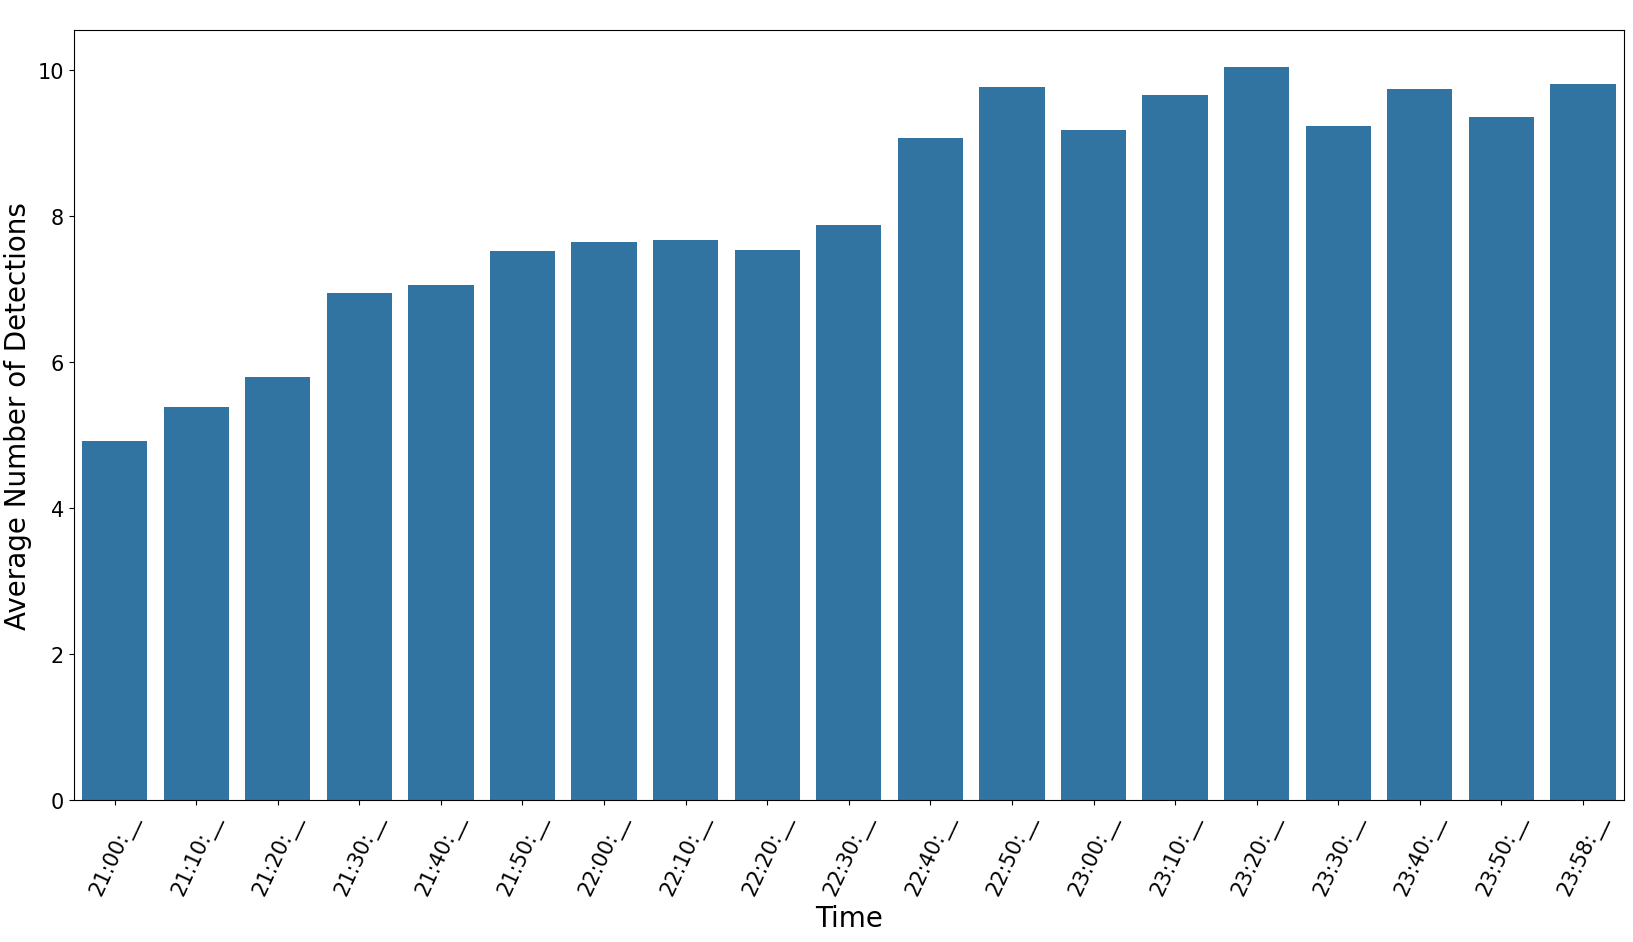
\includegraphics[width=9cm, height=5.5cm]{imgs/detections_final.png}
            \captionsetup{width=0.9\textwidth}
            \caption*{\textbf{Figure 2:} Average number of GroundingDINO insect detections on a trap has at a given time 
            by the general hour and minute.} 
        \end{varwidth}
    \end{figure}

    \tab GroundingDINO, upon manual evaluation, captures insects 
    of different sizes and occassionally misses a very small insect or boxes equipment. While there is no metric on how well
    it fares on detecting insects from Macleish, its number of detections is considered a good proxy for insect activity.
    The detection statistics reveal that there is a peak in insect prescence around time 
    23:20:00 (the images in this cohort are taken at 23:20:03 or 23:20:04), with on average 10.04 insects detected around that time
    (Figure 2). The single specific time in which most insects were classified as moths was 23:50:04 (Figure S4), with around 10 moths predicted per image. 
    However, there were only 3 images
    taken at that time, hence it could be skewed by chance. The number of insects classified as moths seems to be 
    relatively high and stable around 23:10:00 to 23:40:00 (Figure S4). However, the lack of ground truth labels doesn't allow a confident
    answer to when most moths are actually present. Regardless, Mariana and her lab can likely limit insect trap usage to a smaller
    timespan after 11 pm, as the number of insects detected is considerably lower before 11 pm.
    \section{Discussion} 
    \tab The paper contributes a pipeline for annotating images at Macleish: a fine-tuned model that 
     excels in identifying moths from other insects on a separate insect trap dataset, alongside
    another pre-existing model that can retrieve bounding boxes of insects. Combined, these models are used to get 
    statistics on insect detections at Macleish, and classifications on detections for for manual evaluation. More importantly,
    experiments indicate a proof-of-concept that a classifier can reliably identify moths from even a smaller insect crops dataset. This means 
     Macleish images annotations would be a significant supplement moving forward for training a more relevant classifier. 
     And finally, it's discovered that moth traps could be limited to activation at times after 11 pm,
    as that's when most insects were detected. \newline
    \tab The major limitation of this project is 
    the lack of any labelled data on Macleish images. This prevents future
    steps in this project. While insect trap datasets can be similar to Macleish images, Macleish images are unique
    due to the colored lighting the edges of its traps have.
     This paper's moth classifier seems to ambiguously classify insects on image crops saturated by blue
     lighting from the trap. Even among pass @ 5 and pass @ 1 runs, the model detects some crops as moths despite such crops not looking like
     moths (Figure S2 is an example). The pipeline would be significantly improved with annotated Macleish images, ideally with bounding box coordinates. 
     Once that is done, GroundingDINO can be 
     fine-tuned on those coordinates and the classifier would have its AMI-GBIF binary dataset supplemented by Macleish image crops. 
     One assumption that could be formally validated, then, is whether pass @ 5 really does yield better classification accuracy than pass @ 1,
     as pass @ 5 was used due to the assumption that it would be more reliable.
    \newline
    \newline
    \newline
    \\[20\baselineskip]
    \section{References}
    \begin{hangparas}{.25in}{1}
    

    Jain, A., Cunha, F., Bunsen, M. J., Cañas, J. S., Pasi, L., Pinoy, N., Helsing, F., Russo, J., Botham, M., 
    Sabourin, M., Fréchette, J., Anctil, A., Lopez, Y., Navarro, E., Pimentel, F. P., Zamora, A. C., Silva, J. A. R., 
    Gagnon, J., August, T., … Rolnick, D. (2024). Insect identification in the wild: The ami dataset. arXiv.org. 
    https://arxiv.org/abs/2406.12452 
    
    Note: AMI-GBIF Dataset Link: https://zenodo.org/records/11358689 

    Liu, S., Zeng, Z., Ren, T., Li, F., Zhang, H., Yang, J., Jiang, Q., Li, C., Yang, J., Su, H., Zhu, J., 
    \& Zhang, L. (2024). Grounding dino: Marrying dino with grounded pre-training for open-set object detection. 
    Lecture Notes in Computer Science, 38-55. https://doi.org/10.1007/978-3-031-72970-6\_3 \newline 

    Tan, M. \&amp; Le, Q.. (2019). EfficientNet: Rethinking Model Scaling for Convolutional Neural Networks. 
    \textit{Proceedings of the 36th International Conference on Machine Learning},
    in \textit{Proceedings of Machine Learning Research} 
    97:6105-6114. https://doi.org/10.48550/arXiv.1905.11946. 

    \end{hangparas}
    % Jain, A., Cunha, F., Bunsen, M. J., Cañas, J. S., Pasi, L., Pinoy, N., Helsing, F., Russo, J., 
    % Botham, M., Sabourin, M., Fréchette, J., Anctil, A., Lopez, Y., Navarro, E., Pimentel, F. P., Zamora, 
    % A. C., Silva, J. A. R., Gagnon, J., August, T., … Rolnick, D. (2024). Insect identification in the wild:
    %  The ami dataset. arXiv.org. https://arxiv.org/abs/2406.12452 \newline
    % Note: AMI-GBIF Dataset Link: https://zenodo.org/records/11358689 \newline
    % Liu, S., Zeng, Z., Ren, T., Li, F., Zhang, H., Yang, J., Jiang, Q., Li, C., Yang, J., Su, H., Zhu, J., 
    % \& Zhang, L. (2024). Grounding dino: Marrying dino with grounded pre-training for open-set object detection. 
    % Lecture Notes in Computer Science, 38-55. https://doi.org/10.1007/978-3-031-72970-6\_3 \newline 
    % Tan, M. \&amp; Le, Q.. (2019). EfficientNet: Rethinking Model Scaling for Convolutional Neural Networks. 
    % \textit{Proceedings of the 36th International Conference on Machine Learning},
    % in \textit{Proceedings of Machine Learning Research} 
    % 97:6105-6114. https://doi.org/10.48550/arXiv.1905.11946. 


    % \section{References}
    \nobreak

    

% end two column 
\pagebreak 
\onecolumn
\section{Supplementary Materials} 

% 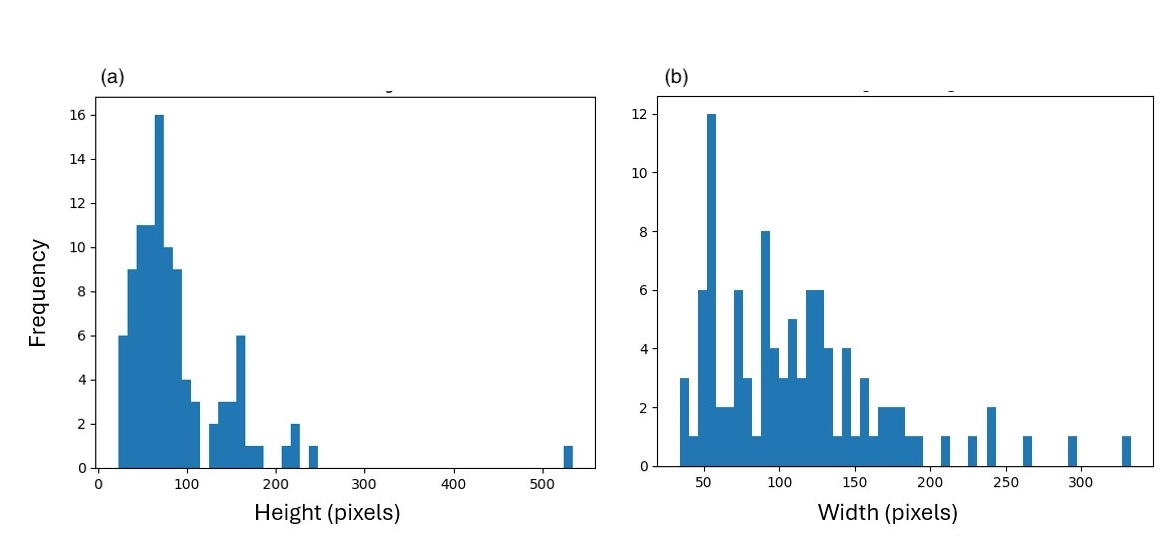
\includegraphics[width=16cm, height=8cm]{imgs/S_fig1.jpg} 
\begin{figure}[h]
        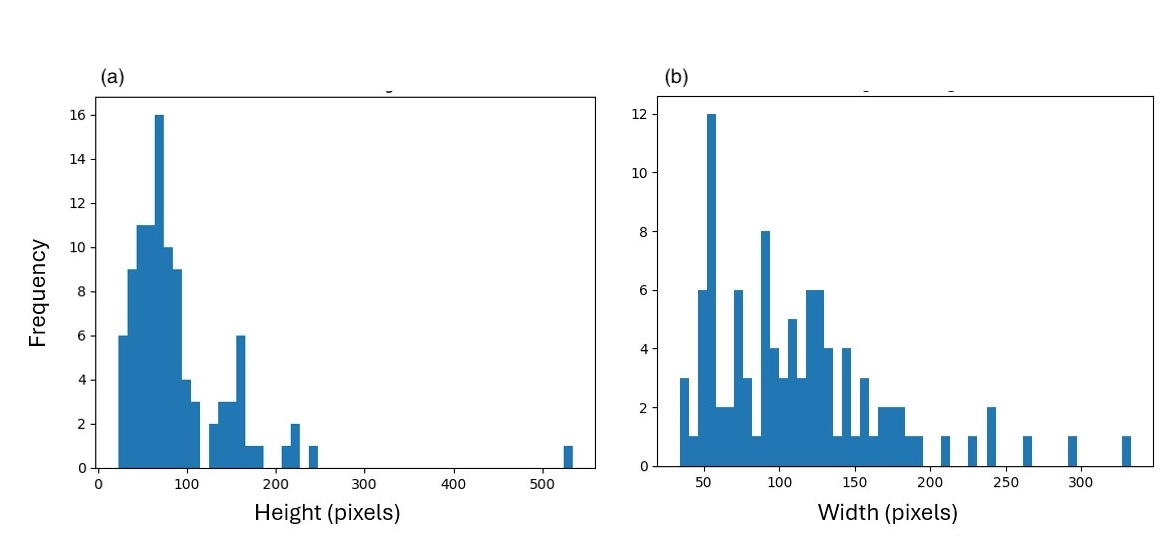
\includegraphics[width=16cm, height=7.5cm]{imgs/S_fig1.jpg}
        \captionsetup{width=0.9\textwidth}
        \caption*{\textbf{Figure S1:} The distribution of image widths (b) and heights (a)
        of 100 randomly sampled images from the AMI-GBIF binary training dataset. Mean 
        width is 89.9 and mean height is 111.6, but there is considerable variation
        (standard deviation above 57 for both)} 
\end{figure} 
\newpage 
\begin{figure}[h]
    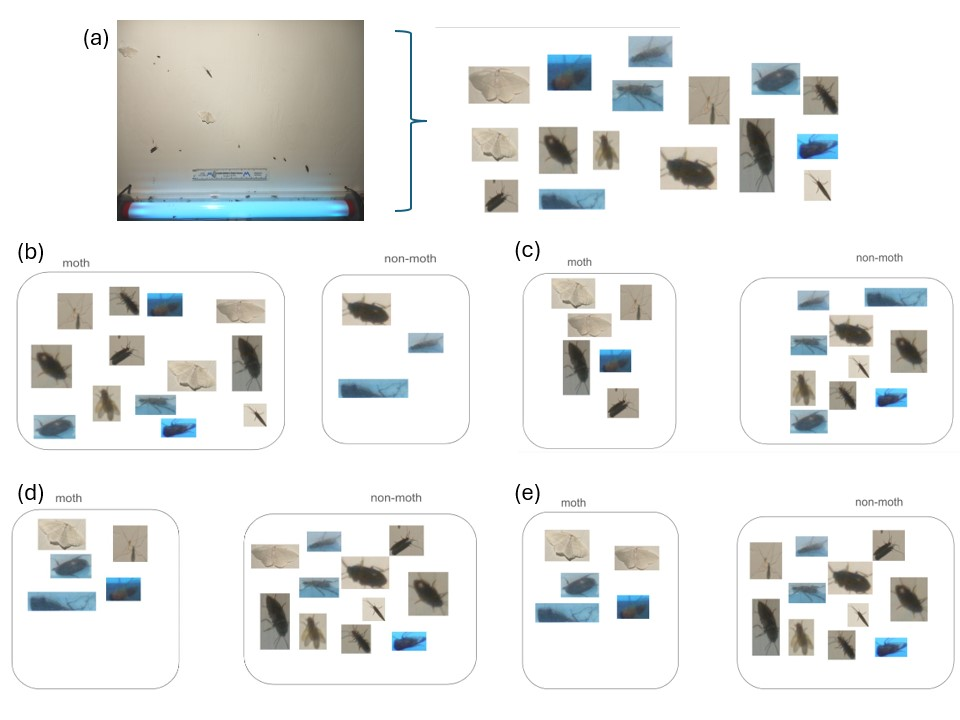
\includegraphics[width=16cm, height=14cm]{imgs/S_fig2.jpg}
    \captionsetup{width=0.9\textwidth}
    \caption*{\textbf{Figure S2:} (a) Some of the image crops generated by GroundingDINO on image 
    ama\_2024-06-17\_23\_00\_04.jpg, barring an incorrect crop on equipment. Ground
    truths of moths vs non-moths aren't known, but speculated. The following predictions are
    done with EfficientNet Full: (b) Results of pass @ 1 predictions
    without reshaping input image crops. With Pass @ 1,
    the model is prompted once and the class with a greater predicted value is chosen.
    (c) The best-performing case of pass @ 5 without reshaping image, where
    the model outputs for the two classes are reshaped via softmax, and then 
    a cutoff of 0.9999 and above is needed for a prediction to be considered 
    ``moth." Without reshaping image crop inputs, the model severely overpredicts moths, and 
    an unreasonably high class cutoff is needed to reduce moth predictions to reasonable amounts. 
    (d) Pass @ 1 predictions with reshaping image to 90 x 110, resulting in a healthy amount of moth
    predictions. (e) Pass @ 5 predictions with reshaping as well. Pass @ 5 with reshape successfully detected both white moths,
     whereas pass @ 1 with reshape only detected one white moth.}  
\end{figure} 
\newpage 
\begin{figure}[h]
    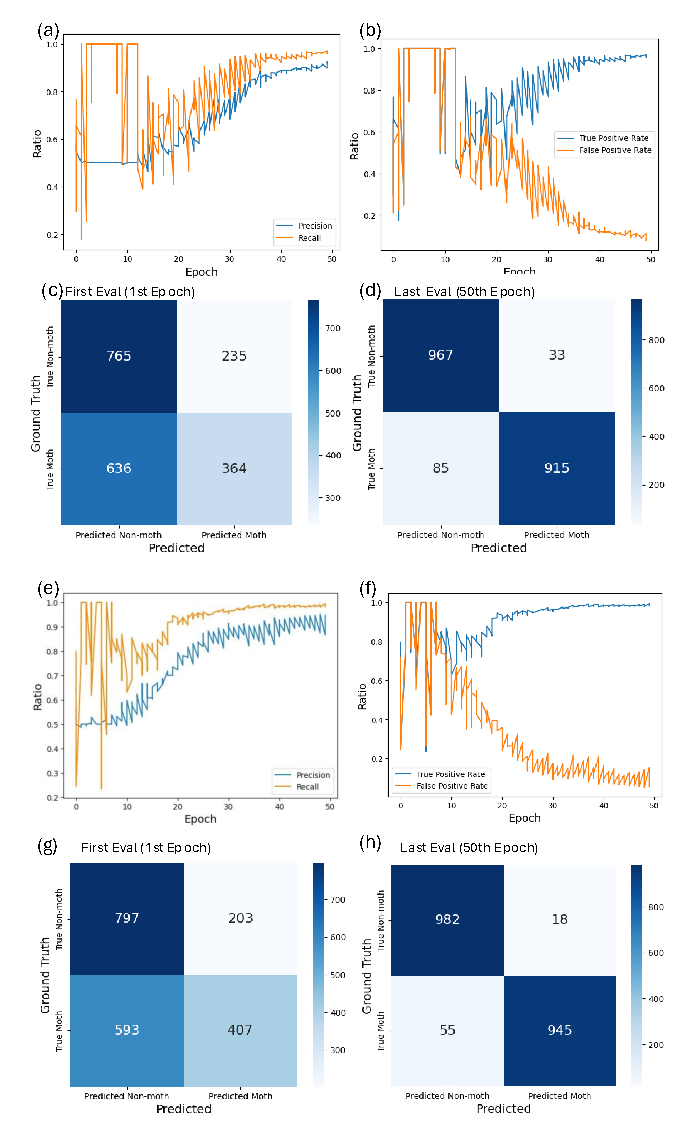
\includegraphics[width=16cm, height=26cm]{imgs/train_summary_crop.pdf}
    % \clearpage 
    % \captionsetup{width=0.9\textwidth}
    % \caption*{\textbf{Figure S1:} The distribution of image widths (b) and heights (a)
    %     of 100 randomly sampled images from the AMI-GBIF binary training dataset. Mean 
    %     width is 89.9 and mean height is 111.6, but there is considerable variation
    %     (standard deviation above 57 for both)}
    % \caption*{\textbf{Figure S3:} Graphs (a) to (d) pertain to
    % training results of EfficientNet Limited} 
\end{figure} 
\clearpage 
\begin{figure}[h]  % continued
    \captionsetup{width=0.9\textwidth}
    \caption*{\textbf{Figure S3:} Graphs (a) to (d) pertain to
    test set results of EfficientNet Limited, while graphs (e) to (h) pertain to EfficientNet Full.
    Testing is done 3 times every epoch, for a total of 50 train epochs. \newline
    (a) and (e) show precision and recall rates throughout training. 
    EfficientNet Limited generally keeps a higher recall than precision, whereas EfficientNet Full has 
    higher overall precision. \newline 
    (b) and (f) show the rates of true positives and false positives throughout training.
    EfficientNet Full and EfficientNet Limited both exhibit the wanted divergence between the two rates,
    with false postitives reaching 0 and true positives reaching 1. \newline
    (c) and (g) show the confusion matrices for the very first test set evaluation of the model. \newline
    (d) and (h) show the confusion matrices for the last test set evaluation of the model. 
    EfficientNet Full has fewer misclassifications than EfficientNet Limited and correctly identifies the
    ground truth class more times.
    \newline
    Both models do well and have similar performance patterns during training.
    } 
\end{figure}
\newpage
\begin{figure}[h]
    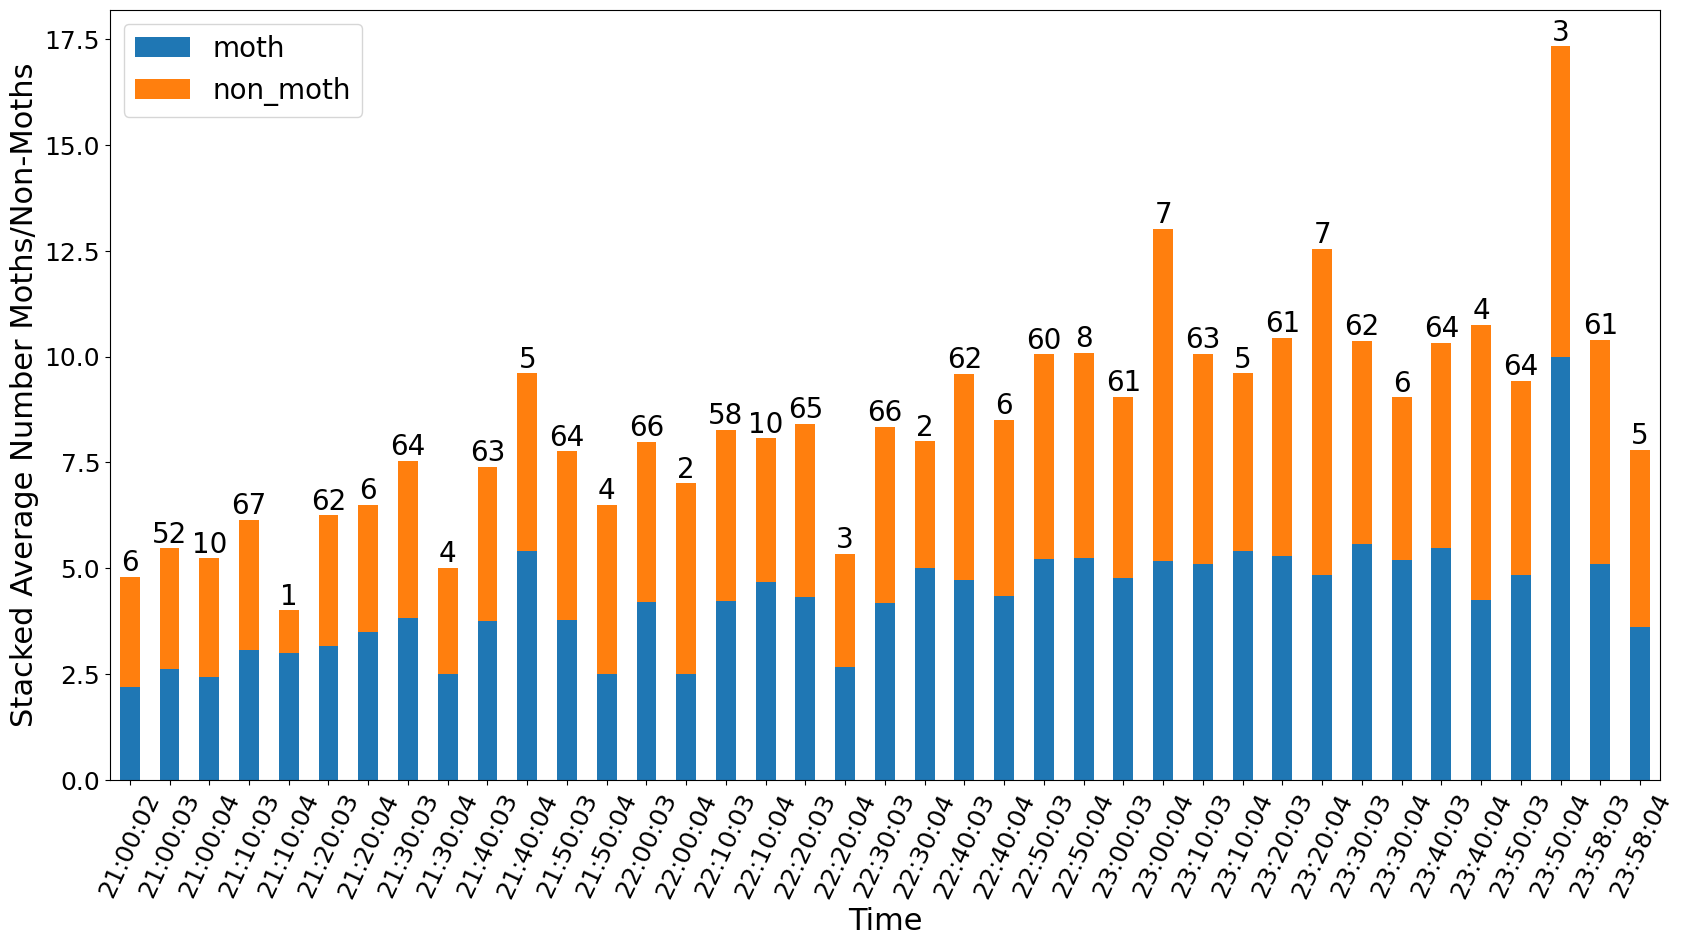
\includegraphics[width=16cm, height=10cm]{imgs/moth_non_moth_final.png}
    \captionsetup{width=0.9\textwidth}
    \caption*{\textbf{Figure S4:} The distribution of moths vs non-moths predicted by 
    EfficientNet Full pass @ 5 from insect detection crops of Macliesh images, averaged by total number of images taken at a specific time.
    The number of images that were taken at a particular time are at the top of each bar.
    % The time 23:50:04 is an outlier time when most insects and moths are detected,
    % averaging to around 10 moths per image, but there are only 3 photos at that time.
     Of course, due to lack of ground truth labels, this shouldn't be taken as a definitive 
    nor accurate conclusion about when most moths are present.} 
\end{figure} 
\end{document}
